
\chapter{Introdução}
 
A atual arquitetura de rede da Internet é composta por: nós de comutação (roteadores e switches, responsáveis pelo encaminhamento de pacotes de dados) e os hosts (máquinas de origem e destino de pacotes de dados, como computadores de usuários, servidores, smartphones, etc). Os nós de comutação possuem uma tabela que os indica qual é o próximo nó que um pacote deve ser encaminhado , chamada de tabela de encaminhamento. Como um pacote pode passar por múltiplos nós até chegar ao seu destino, e como o fluxo de pacotes em cada nó é extremamente alto, toda a operação de consulta a tabela de encaminhamento e transmissão de dados é realizado via hardware. Como o exemplo (Figura \ref{Fig_Rede}) onde observa-se uma rede de Internet de maneira simplificada .

\begin{figure}[h]
\centering
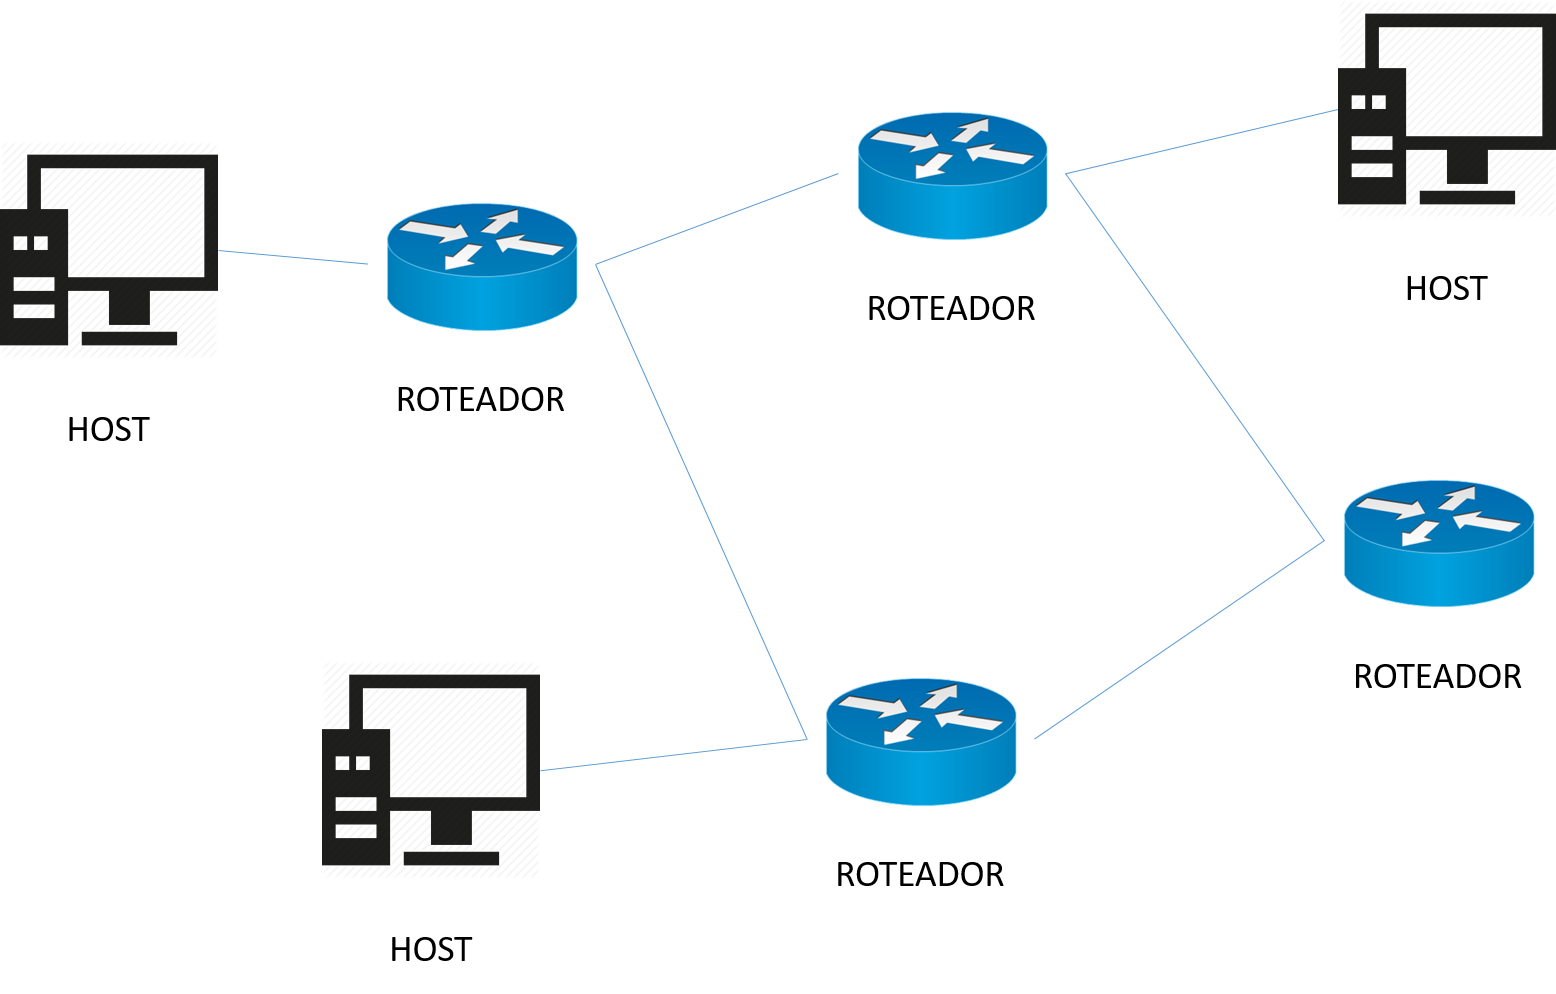
\includegraphics[width=0.7\textwidth]{Introducao/Rede.png}
\caption{Estrutura de uma Rede}
\label{Fig_Rede}
\end{figure}

Essa estrutura se mostrou extremamente eficiente, e permitiu que a expansão em nível mundial da Internet, uma vez que diversas redes com tamanhos e topologias diferentes conseguem se comunicar. 

Proporcional à expansão da Internet e a criação de cada vez mais dispositivos capazes de usá-la, houve um grande aumento no fluxo de dados. Tal aumento advém de práticas como o consumo de vídeo, através de plataformas como Youtube, Netflix, etc, sendo este o tipo de dado mais consumido e o segundo que mais cresce desde 2017\cite{CISCO}

Portanto, devido a essa progressiva demanda, novas arquiteturas de rede estão sendo investigadas. Contudo, como o núcleo da arquitetura atual, ou seja, os nós de comutação, são implementados via hardware, a implementação de arquiteturas experimentais se torna pouco viável, devido aos grandes custos dessa mudança de hardware, além do fato que essa troca iria interromper o fluxo de produção atual de uma rede, fator que dificulta o teste e validação de novas arquiteturas em ambientes reais, principalmente em redes de larga escala.

Dessa forma, soluções baseadas em software se tornaram mais atraentes devido a possibilidade de serem implementadas sem troca de hardware e sem interrupção da rede. Uma dessas alternativas que tem ganhado destaque é o paradigma SDN(Software Defined NetWork) juntamente com o protocolo OpenFlow. Uma rede SDN, utiliza de um dispositivo chamado controlador, que se conecta a todos os nós da rede, para configurá-los de acordo com o gerente da rede. O protocolo Openflow é um protocolo voltado para as redes SDN, que permite que o controlador se comunique com os comutatores.

A implementação de redes SDN ainda está numa fase experimental, e por isso, diversas pesquisas estão sendo desenvolvidas para verificar a performance desse tipo de rede. Uma das grandes vantagens de uma rede SDN é a possibilidade de separar o tráfego de dados em fluxos diferentes, além de poder alterar a tabela de encaminhamento dos comutatores para atingir um melhor desempenho da rede. 

Dessa forma, o objetivo desse trabalho é a criação de uma aplicação capaz de monitorar o fluxo de uma rede e identificar o consumo de dados de vídeos, provenientes de duas das principais plataformas de streaming : Youtube e NetFlix. Essa aplicação será integrada a um tipo de controlador chamado POX e testada através de software capaz de simular redes fisicas, chamado Mininet. Os conceitos de SDN , protocolo OpenFlow e controlador POX serão explicados de forma mais detalhada no capítulo 2.

\section{Objetivos}
\subsection{Objetivo geral}
Implementar e avaliar o desempenho de uma aplicação de monitoramento e classificação de fluxos de dados, utilizando uma rede SDN , junto com um controlador do tipo POX.

\subsection{Objetivos Específicos}

\begin{itemize}
\item Criar e configurar um ambiente de rede SDN, onde seja possível gerar e capturar todo o tráfego da rede. 
\item Implementar um módulo de monitoramento do tráfego da rede, para análise posterior.
\item Implementar o módulo de identificação e classificação do tipo de dados que trafega pela rede.
\item Implementar um módulo de detecção e tratamento de falhas na rede, para que a aplicação possa priorizar um determino tipo de fluxo.
\item Utilizar um banco da dados SQL, para armazenar todos os dados gerados pela aplicação
\end{itemize}3
\section{Estrutura do Trabalho}
Este trabalho será estruturado em 5 capítulos. No capítulo 2 serão explicados mais profundamente os conceitos de paradigma SDN, protoloco OpenFlow, controlador POX, além de das estruturas da arquitetura atual da Internet. Os módulos criados para a aplicação, suas funcionalidades, especificações, e ferramentas utilizadas serão apresentados no capitulo 3, assim como o ambiente em que o módulo foi testado.

O capítulo 4 será feita uma exposição e análise dos resultados obtidos. E por fim, no capítulo 5 serão expostas as conclusões, considerações finais e trabalhos futuros.


